\documentclass[noauthor,nooutcomes,hints,handout]{ximera}

\graphicspath{  
{./}
{./whoAreYou/}
{./drawingWithTheTurtle/}
{./bisectionMethod/}
{./circles/}
{./anglesAndRightTriangles/}
{./lawOfSines/}
{./lawOfCosines/}
{./plotter/}
{./staircases/}
{./pitch/}
{./qualityControl/}
{./symmetry/}
{./nGonBlock/}
}


%% page layout
\usepackage[cm,headings]{fullpage}
\raggedright
\setlength\headheight{13.6pt}


%% fonts
\usepackage{euler}

\usepackage{FiraMono}
\renewcommand\familydefault{\ttdefault} 
\usepackage[defaultmathsizes]{mathastext}
\usepackage[htt]{hyphenat}

\usepackage[T1]{fontenc}
\usepackage[scaled=1]{FiraSans}

%\usepackage{wedn}
\usepackage{pbsi} %% Answer font


\usepackage{cancel} %% strike through in pitch/pitch.tex


%% \usepackage{ulem} %% 
%% \renewcommand{\ULthickness}{2pt}% changes underline thickness

\tikzset{>=stealth}

\usepackage{adjustbox}

\setcounter{titlenumber}{-1}

%% journal style
\makeatletter
\newcommand\journalstyle{%
  \def\activitystyle{activity-chapter}
  \def\maketitle{%
    \addtocounter{titlenumber}{1}%
                {\flushleft\small\sffamily\bfseries\@pretitle\par\vspace{-1.5em}}%
                {\flushleft\LARGE\sffamily\bfseries\thetitlenumber\hspace{1em}\@title \par }%
                {\vskip .6em\noindent\textit\theabstract\setcounter{question}{0}\setcounter{sectiontitlenumber}{0}}%
                    \par\vspace{2em}
                    \phantomsection\addcontentsline{toc}{section}{\thetitlenumber\hspace{1em}\textbf{\@title}}%
                     }}
\makeatother



%% thm like environments
\let\question\relax
\let\endquestion\relax

\newtheoremstyle{QuestionStyle}{\topsep}{\topsep}%%% space between body and thm
		{}                      %%% Thm body font
		{}                              %%% Indent amount (empty = no indent)
		{\bfseries}            %%% Thm head font
		{)}                              %%% Punctuation after thm head
		{ }                           %%% Space after thm head
		{\thmnumber{#2}\thmnote{ \bfseries(#3)}}%%% Thm head spec
\theoremstyle{QuestionStyle}
\newtheorem{question}{}



\let\freeResponse\relax
\let\endfreeResponse\relax

%% \newtheoremstyle{ResponseStyle}{\topsep}{\topsep}%%% space between body and thm
%% 		{\wedn\bfseries}                      %%% Thm body font
%% 		{}                              %%% Indent amount (empty = no indent)
%% 		{\wedn\bfseries}            %%% Thm head font
%% 		{}                              %%% Punctuation after thm head
%% 		{3ex}                           %%% Space after thm head
%% 		{\underline{\underline{\thmname{#1}}}}%%% Thm head spec
%% \theoremstyle{ResponseStyle}

\usepackage[tikz]{mdframed}
\mdfdefinestyle{ResponseStyle}{leftmargin=1cm,linecolor=black,roundcorner=5pt,
, font=\bsifamily,}%font=\wedn\bfseries\upshape,}


\ifhandout
\NewEnviron{freeResponse}{}
\else
%\newtheorem{freeResponse}{Response:}
\newenvironment{freeResponse}{\begin{mdframed}[style=ResponseStyle]}{\end{mdframed}}
\fi



%% attempting to automate outcomes.

%% \newwrite\outcomefile
%%   \immediate\openout\outcomefile=\jobname.oc
%% \renewcommand{\outcome}[1]{\edef\theoutcomes{\theoutcomes #1~}%
%% \immediate\write\outcomefile{\unexpanded{\outcome}{#1}}}

%% \newcommand{\outcomelist}{\begin{itemize}\theoutcomes\end{itemize}}

%% \NewEnviron{listOutcomes}{\small\sffamily
%% After answering the following questions, students should be able to:
%% \begin{itemize}
%% \BODY
%% \end{itemize}
%% }
\usepackage[tikz]{mdframed}
\mdfdefinestyle{OutcomeStyle}{leftmargin=2cm,rightmargin=2cm,linecolor=black,roundcorner=5pt,
, font=\small\sffamily,}%font=\wedn\bfseries\upshape,}
\newenvironment{listOutcomes}{\begin{mdframed}[style=OutcomeStyle]After answering the following questions, students should be able to:\begin{itemize}}{\end{itemize}\end{mdframed}}



%% my commands

\newcommand{\snap}{{\bfseries\itshape\textsf{Snap!}}}
\newcommand{\flavor}{\link[\snap]{https://snap.berkeley.edu/}}
\newcommand{\mooculus}{\textsf{\textbf{MOOC}\textnormal{\textsf{ULUS}}}}


\usepackage{tkz-euclide}
\tikzstyle geometryDiagrams=[rounded corners=.5pt,ultra thick,color=black]
\colorlet{penColor}{black} % Color of a curve in a plot



\ifhandout\newcommand{\mynewpage}{\newpage}\else\newcommand{\mynewpage}{}\fi


\author{Bart Snapp}

\title{Seven types of frieze patterns}

\begin{document}
\begin{abstract}
  How many different frieze patterns can we have with different combinations of  types of symmetries?
\end{abstract}
\maketitle

\begin{listOutcomes}
\item List all possible symmetries of frieze patterns.
\item Recognize when certain symmetries follow from compositions of
  other symmetries.
\item Organize frieze patterns by their symmetries.
\end{listOutcomes}



Let's categorize our frieze patterns by the symmetries they have. Let
\begin{itemize}
  \item $\{T\}$ be the set of frieze patters with symmetries through
    translations and and no others.
  \item $\{T,G\}$ be the set of frieze patters with symmetries through
    translations, glide-reflections, and and no others.
  \item $\{T,R\}$ be the set of frieze patters with symmetries through
    translations, $180^\circ$ rotations, and and no others.
  \item $\{T,V_h\}$ be the set of frieze patters with symmetries
    through translations, horizontal-reflections, and and no
    others.
  \item $\{T,G,F_v,F_h,R\}$ be the set of frieze patterns with maximal
    symmetry.
\end{itemize}
Let's try to visualize the relations between the symmetries of the
frieze patterns by drawing a diagram
\begin{center}
  \begin{tikzcd}
    & \{T,G,R,F_v,F_h\} \ar[ld,-]\ar[rd,-] \ar[d,-]&       \\
    {} &        {}        &  {} \\
    {} &   {\resizebox{.5in}{!}{?}}                 & \\
    {} &        {}          &  {} \\
    \{T,G\}\ar[u,-]\ar[rd,-] & \{T,R\}\ar[d,-]\ar[u,-] & \{T,F_h\}\ar[ld,-]\ar[u,-]       \\   
    & \{T\} &
  \end{tikzcd}
\end{center}
We know what is happening at the top and bottom, but the middle is
more mysterious. We'll figure that out NOW.




\mynewpage


\begin{question}
  List all possible combinations of the TYPES of symmetries that
  frieze patterns can have.
  \begin{freeResponse}
    There are a total of $16 = 2^4$ combinations of TYPES of
    symmetries for frieze patterns. This is because EVERY frieze
    pattern has symmetry through translations, and there are $4$ other
    TYPES of symmetry a frieze pattern can have.  Now let's list the
    $16$ possibilities.
    \begin{itemize}
    \item With one TYPE of symmetry: $\{T\}$
    \item With two TYPES of symmetry: $\{T,G\}$, $\{T,R\}$, $\{T,F_h\}$, $\{T,F_v\}$
    \item With three TYPES of symmetry: $\{T,G,R\}$, $\{T,G,F_h\}$, $\{T,G,F_v\}$, $\{T,R,F_h\}$, $\{T,R,F_v\}$, $\{T,F_v,F_h\}$
    \item With four TYPES of symmetry:  $\{T,G,R,F_h\}$, $\{T,G,R,F_v\}$, $\{T,G,F_v,F_h\}$, $\{T,R,F_v,F_h\}$
    \item With five TYPES of symmetry: $\{T,G,R,F_v,F_h\}$
    \end{itemize}
  \end{freeResponse}
\end{question}
\mynewpage

\begin{question}
  Which of the possible combinations are actually the SAME collection
  of symmetries?
  \begin{freeResponse}
    From our previous work, we have the following TYPE-multiplication table:
    \[\renewcommand{\arraystretch}{2}
    \begin{array}{|c||c|c|c|c|c|}
      \hline
      & T    & R    & F_h   & F_v & G     \\ \hline\hline
      T   & T    & R   & F_h    & G   & G     \\ \hline
      R   & R   & T    & G    & F_h & F_h   \\ \hline
      F_h & F_h   & G   & T     & R   & R   \\ \hline
      F_v & G    & F_h  & R     & T   & T   \\ \hline
      G   & G    & F_h  & R     & T   & T   \\ \hline
    \end{array}
    \]
    From the table we can see that:
    \begin{itemize}
      \item Frieze patterns with symmetries through one of 
        \[
        \{T,G,R,F_v\}, \quad  \{T,G,F_v,F_h\}, \quad \{T,R,F_v,F_h\}, \quad \{T,R,F_v\}, \quad \{T,F_v,F_h\}
        \]
        must have symmetries through $\{T,G,R,F_v,F_h\}$.
      \item Frieze patterns with symmetries through one of
        \[
        \{T,G,R\}, \quad \{T,G,F_h\}, \quad \{T,R,F_h\}
        \]
        must have symmetries through $\{T,G,R,F_h\}$.
      \item Frieze patterns with symmetries through $\{T,F_v\}$ must have symmetries through $ \{T,G,F_v\}$.
    \end{itemize}
  \end{freeResponse}
\end{question}
\mynewpage


\begin{question}
  Let's put this together:
  \begin{enumerate}
  \item Complete the diagram that we began with.
  \item Give a representative frieze pattern for each combination of symmetry TYPES.
  \item EXPLAIN why someone might say that there are only ``seven
    types'' of frieze patterns.
  \end{enumerate}
  \begin{freeResponse}
    \begin{enumerate}
    \item Here is my chart:
      \begin{center}
      \begin{tikzcd}[column sep=-1em]
        & \begin{minipage}{3.5in}
            \begin{center}
              $\{T,G,R,F_v,F_h\}$ \tiny\\
              $=  \{T,G,R,F_v\}=  \{T,G,F_v,F_h\}=\{T,R,F_v,F_h\}  = \{T,R,F_v\}=\{T,F_v,F_h\}$
          \end{center}\end{minipage} \ar[ldd,-]\ar[rd,-] &       \\
    {} &        {}           &  \begin{minipage}{1.5in}
      \begin{center}$\{T,G,R,F_h\}$\tiny\\
        $=\{T,G,R\} =\{T,G,F_h\}=\{T,R,F_h\}$
      \end{center}
    \end{minipage}
    \\
    \begin{minipage}{1in}
      \begin{center}$\{T,G,F_v\}$\tiny\\
        $= \{T,F_v\}$ 
      \end{center}
    \end{minipage}
&                &  {} \\
    \{T,G\}\ar[u,-]\ar[rd,-] \ar[rruu,-]& \{T,R\}\ar[d,-]\ar[ruu,-] & \{T,F_h\}\ar[ld,-]\ar[uu,-]       \\   
    & \{T\} &
  \end{tikzcd}
      \end{center}
    \item REPRESENTATIVES:
      \begin{description}
      \item[$\{T\}$:]\raisebox{-.45\height}{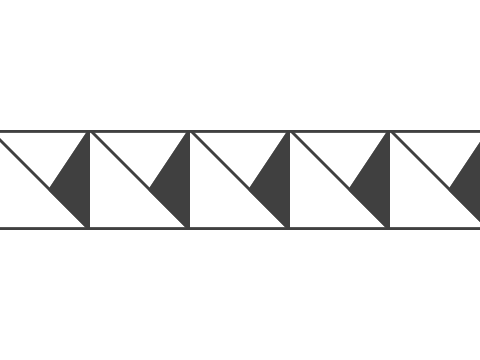
\includegraphics[width=.3\textwidth]{7T.png}}
      \item[$\{T,G\}$:]\raisebox{-.45\height}{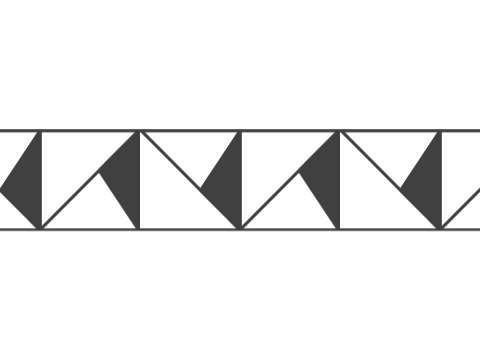
\includegraphics[width=.3\textwidth]{7TG.png}}
      \item[$\{T,R\}$:]\raisebox{-.45\height}{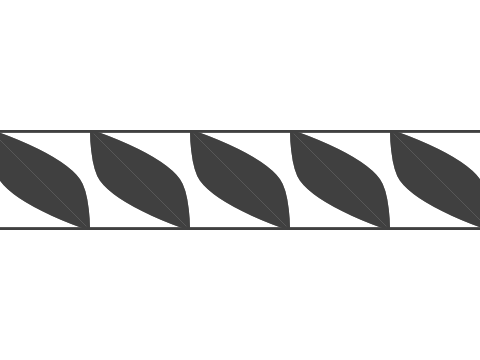
\includegraphics[width=.3\textwidth]{7TR.png}}
      \item[$\{T,F_h\}$:]\raisebox{-.45\height}{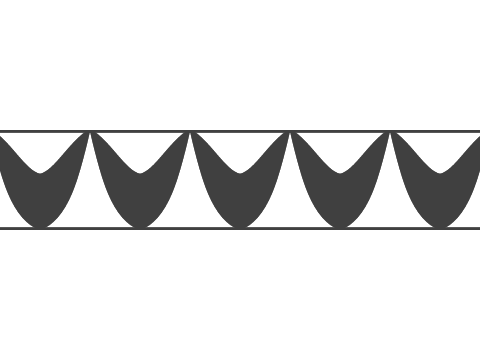
\includegraphics[width=.3\textwidth]{7TF.png}}
      \item[$\{T,G,F_v\}$:]\raisebox{-.45\height}{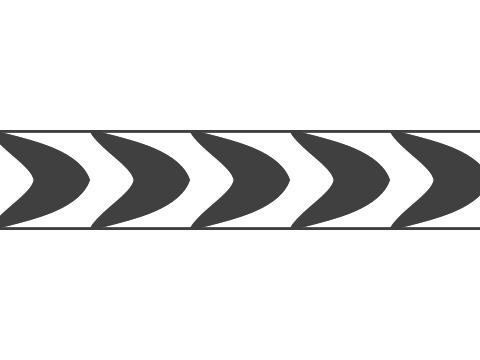
\includegraphics[width=.3\textwidth]{7TGF.png}}
      \item[$\{T,G,R,F_h\}$:]\raisebox{-.45\height}{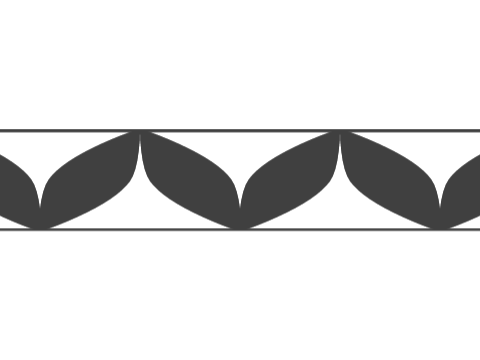
\includegraphics[width=.3\textwidth]{7TGRF.png}}
      \item[$\{T,G,R,F_v,F_h\}$:]\raisebox{-.45\height}{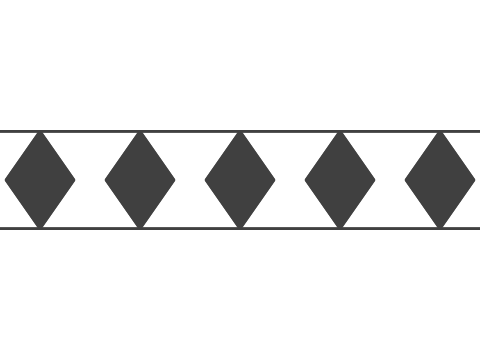
\includegraphics[width=.3\textwidth]{7TGRFF.png}}
      \end{description}
    \item Since there are only $7$ types of combinations of symmetry
      for frieze patterns, someone might say there are only seven
      types.
    \end{enumerate}
  \end{freeResponse}
\end{question}

\end{document}
